\documentclass[11pt]{article}
\usepackage[margin=1in]{geometry}
\usepackage{amsmath,amssymb}
\usepackage{tikz}
\usepackage{float}
\usepackage{graphicx}
\usepackage[hidelinks]{hyperref}

\setlength{\parindent}{0pt}
\setlength{\parskip}{0.7\baselineskip}

\begin{document}

\section{Other (More Specific) Kinds of Solvers and Encodings}

Why talk about these?
\begin{itemize}
    \item To give you an idea of what's out there, and different kinds of encodings.
    \item To give you something to compare to.
\end{itemize}

We will talk about:
\begin{itemize}
    \item \textbf{Integer programs}
    \item SAT solvers
    \item Stochastic and local search (next time)
\end{itemize}

And how we might compare the performance of different solvers or techniques.

\subsection{Integer programming}

We have in a sense already done some integer programming, just encoded as CSPs in MiniZinc style.

An integer program is a mathematical optimisation in which the variables are integers (if you've seen linear programming before, it's a linear program where we restrict variables to integer values).
\begin{itemize}
    \item Often people actually mean integer \emph{linear} programming, where the constraints are linear.
    \item If some of the variables are not integers, we have \emph{mixed-integer} programming (MIP).
    \item If the integer domains are restricted to subsets of $\{0, 1\}$ then we call it zero-one, or binary, integer programming.
\end{itemize}

\paragraph{How do we encode a problem as an ILP?} Learn by examples.

\subsubsection{Knapsack example}

We are a child running away from home, and are packing a knapsack of snacks. Each snack has a cost in terms of backpack space (or weight maybe), and a desirability. We want to optimise our desirability subject to space. We have:
\begin{itemize}
    \item apples ($a$): cost 3, gain 4;
    \item lettuces ($l$): cost 7, gain 2;
    \item carrots ($c$): cost 4, gain 2.
\end{itemize}

So we want to maximise
\[
    4a + 2l + 2c
\]
subject to
\[
    3a + 7l + 4c \leq \text{capacity}.
\]

\subsubsection{Graph colouring example}

We have a graph $G = (V, E)$ and we want to colour it with a minimum number of colours. We need a number of variables and constraints.

\textbf{(Boolean) Variables:}
\begin{itemize}
    \item For each vertex $i$ and colour $j$:
    \begin{itemize}
        \item $c_{i,j}$ is $1$ if vertex $i$ is colour $j$, $0$ otherwise;
        \item $w_j$ is $1$ if we use colour $j$, $0$ otherwise.
    \end{itemize}
    \item The domain of $i$ is the set of vertices, and the domain of $j$ is the set of colours.
\end{itemize}

\textbf{Objective function:}
\[
    \min \sum_{j} w_j
\]

\textbf{Subject to constraints:}
\begin{itemize}
    \item Every node gets exactly one colour:
    \[
        \forall i \in V,\quad \sum_{j} c_{i,j} = 1.
    \]
    \item Every edge has different-coloured ends:
    \[
        \forall (u, v) \in E,\ j \in C,\quad c_{u,j} + c_{v,j} \leq 1.
    \]
    \item We record when we use a colour:
    \[
        \forall i \in V,\ j \in C,\quad c_{i,j} \leq w_j.
    \]
\end{itemize}

\subsubsection{A nice example using OR-Tools}

A worked example is available as a \href{https://colab.research.google.com/drive/1Gxt_sBVOZAaUo_LNvz60e1BacJ_azivs?usp=sharing}{Colab notebook}, adapted from this \href{https://phabe.ch/2023/08/07/vertex-coloring-using-ilp/}{blog post}.

That's from a student who was taking a course at Bonn -- the deep-dive notes on that section are in these \href{https://www.or.uni-bonn.de/~held/hausdorff_school_22/slides/GraphColoringFormulations.pdf}{slides}, if you're interested.

And if you're \emph{really} keen, here's a \href{https://arxiv.org/pdf/1706.10191}{related paper}.

\subsubsection{A PuLP in Python example}

See this \href{https://colab.research.google.com/drive/1_PIERNAIiQbVuDekkfdIkLQGtY2-dm4m?usp=sharing}{Colab notebook}.

\subsubsection{An ILP for firefighting}

\textbf{Firefighting problem:} a fire breaks out on a graph $G = (V, E)$ at vertex $r$. On each turn we get to defend $d$ vertices. Then the fire spreads to all non-burning, non-defended vertices that are adjacent to a burning vertex. Burning vertices burn forever, defended vertices are defended forever.

Questions:
\begin{itemize}
    \item \textbf{Decision version:} can we save some specified proportion of the graph (or number of vertices)?
    \item \textbf{Optimisation version:} what is the maximum number of vertices we can save?
\end{itemize}

A few resources:
\begin{itemize}
    \item a classic survey: A.\ Finbow and G.\ MacGillivray, ``The Firefighter Problem: A survey of results, directions and questions,'' \emph{Australasian Journal of Combinatorics}, 43 (2009), 57--77.
    \item a paper about ILP and heuristic techniques on this problem: \url{https://dl.acm.org/doi/10.1016/j.cor.2015.02.004}.
\end{itemize}

We can encode this as an ILP.

Some notation:
\begin{itemize}
    \item $G = (V, E)$ is the graph;
    \item $T$ is some maximum time;
    \item $N(x)$ is the neighbourhood of vertex $x$;
    \item we'll use $t$ to denote times;
    \item $r_i$ are the places the fire starts, for $1 \leq i \leq f$;
    \item $f$ is the number of vertices where the fire starts;
    \item $d$ is our budget of defenders.
\end{itemize}

Some variables and how we interpret them:
\begin{itemize}
    \item $b_{x,t}$ gets $1$ if vertex $x$ is burned at or before $t$, $0$ otherwise;
    \item $d_{x,t}$ gets $1$ if vertex $x$ is defended at or before $t$, $0$ otherwise.
\end{itemize}

\begin{figure}[H]
    \centering
    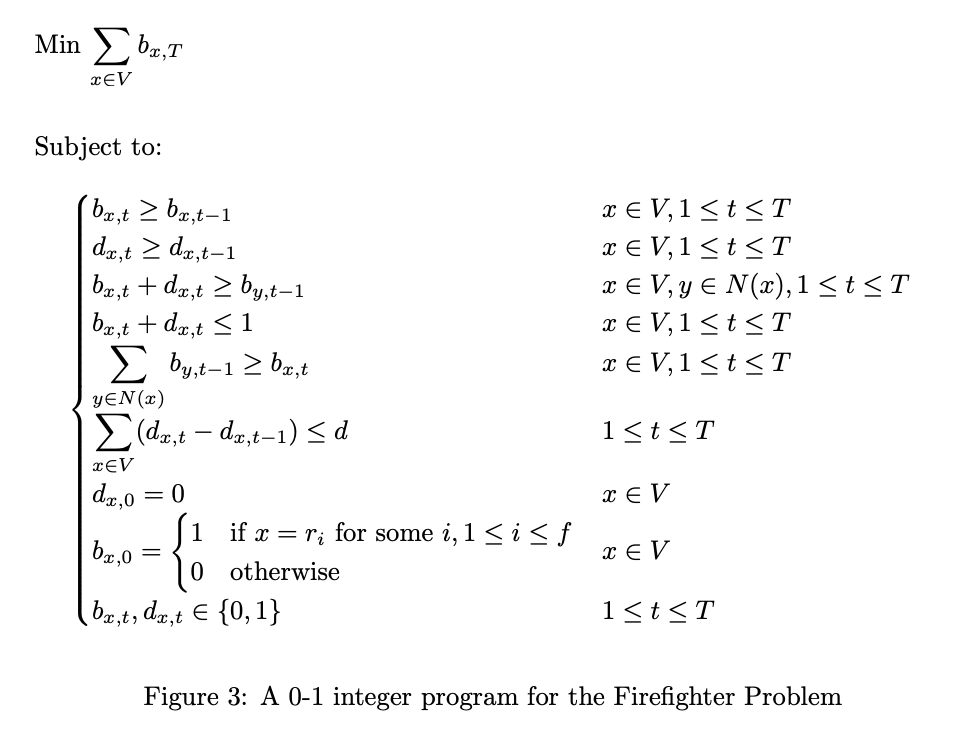
\includegraphics[width=0.75\textwidth]{image.png}
    \caption{A 0-1 integer program for the Firefighter Problem.}
\end{figure}

\subsubsection{How do we solve ILPs}

In many cases, similar ways to how we solve CPs -- branch and bound is popular.

But there's an additional bit that we can take advantage of: linear relaxations. A linear relaxation of an integer program is a version of the program where we do not require the variables to be integers (they could instead be real numbers).

Why would we do this?
\begin{itemize}
    \item Solving ILPs is NP-hard.
    \item Solving this kind of LPs is polynomial-time.
\end{itemize}

Why does this not solve our problem?
\begin{itemize}
    \item Rounding the relaxation doesn't necessarily give us a solution (the difference is something called the \textbf{integrality gap}).
\end{itemize}

So why is it useful at all?
\begin{itemize}
    \item The solution to a relaxation can tell us things about possible solutions to the original ILP.
\end{itemize}

In particular, the solution to the relaxation is \emph{as good or better} than the best solution to the ILP: if it's a maximisation it's the same or bigger, if it's a minimisation it's the same or smaller.

Let's look at a picture from Wikipedia:

\begin{figure}[H]
    \centering
    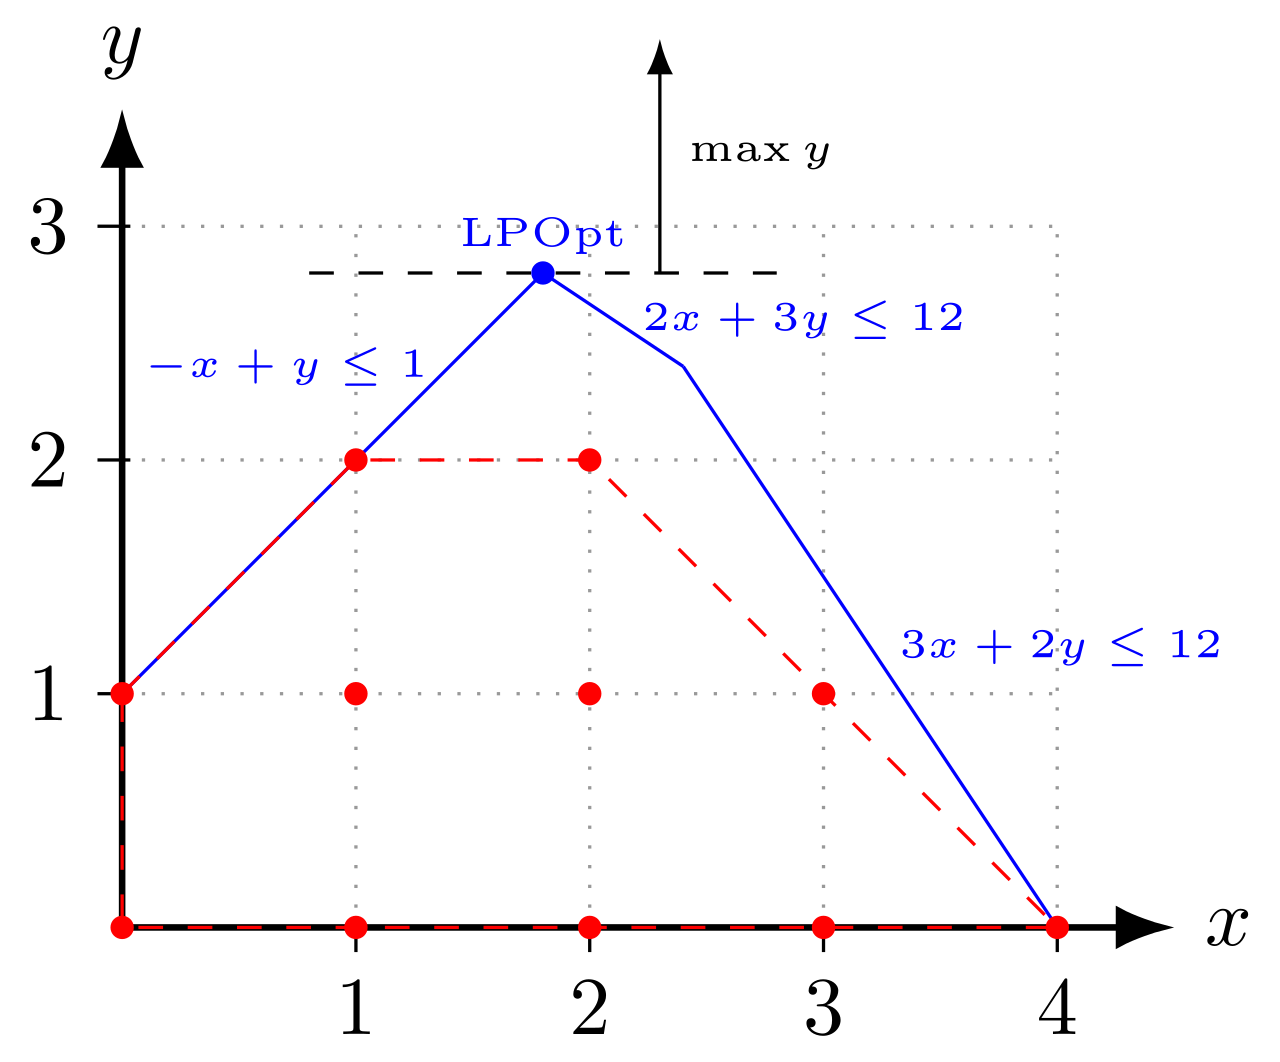
\includegraphics[width=0.6\textwidth]{image-1.png}
    \caption{Polytopes of all feasible integer points and of the LP relaxation to the integer linear program $\max\{\, y \mid {-x+y\leq 1};\ 3x+2y\leq 12;\ 2x+3y\leq 12;\ x,y\in Z_+ \,\}$. \emph{(CC-BY; Fanosta -- derivative work based on ``IP polytope with LP relaxation.png'' by Sdo.)}}
\end{figure}

(Extra thing to note: how visible the linear nature of the constraints is here.)

This bound helps us in pruning during search.

\subsection{SAT solvers}

Satisfiability solvers deal specifically in solving propositional-logic expressions of the sort we've seen in our examples of, e.g., 3-CNF-SAT.

Note that one of the fastest CP solvers around currently is based on a SAT solver: \href{https://developers.google.com/optimization/cp/cp_solver}{Google OR-Tools CP-SAT}. It does pretty well in the \href{https://www.minizinc.org/challenge.html}{MiniZinc Challenge}.

Various solver approaches exist, and often combination ones work out the best. We'll outline a few.

\subsubsection{Davis--Putnam--Logemann--Loveland (DPLL) algorithm}

\begin{figure}[H]
    \centering
    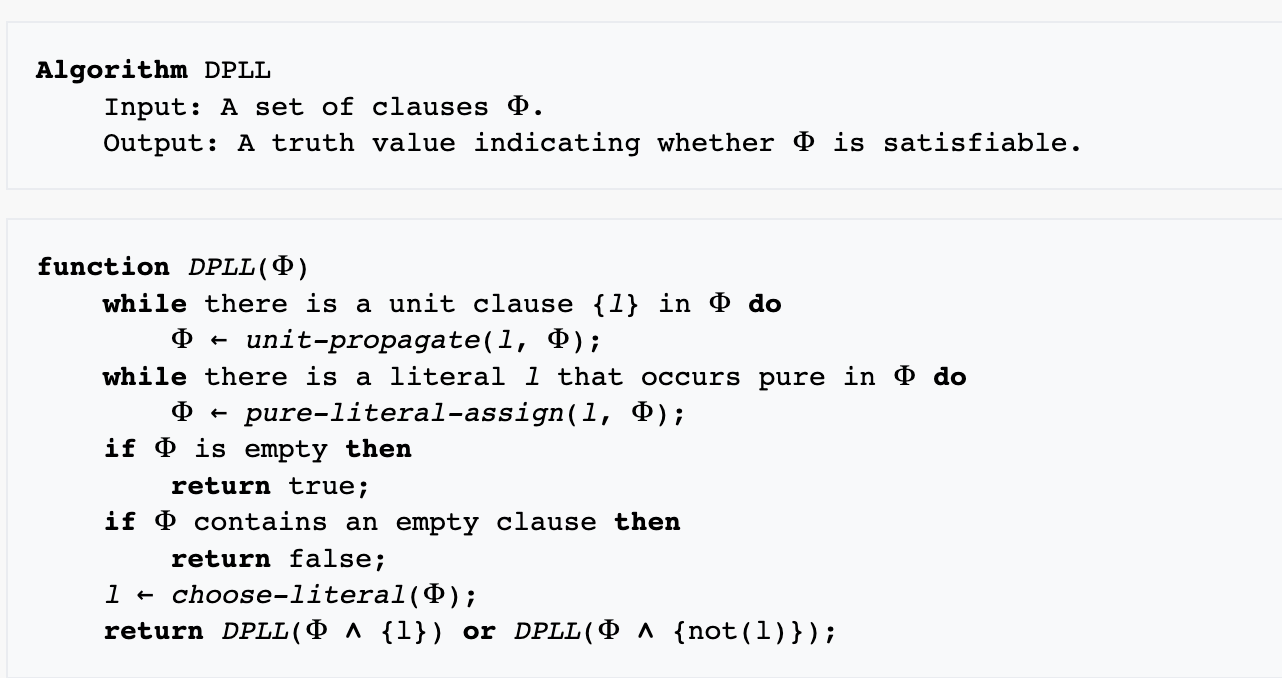
\includegraphics[width=0.85\textwidth]{image-2.png}
    \caption{Pseudocode for the DPLL algorithm (from Wikipedia).}
\end{figure}

\begin{itemize}
    \item Unit propagation is something we can do when a clause has only one literal -- it is a \emph{unit clause}. Then we know that literal must be satisfied, and so we can record that, remove any clause with that literal in it, and remove the negation of the literal from any clause.
    \item Pure literal assignment is something we do when a variable only appears as a positive or only as a negative literal. Then we can assign the value that satisfies that literal and remove any clause with it in.
\end{itemize}

\subsubsection{Randomized algorithms}

Randomized or probabilistic algorithms (e.g.\ Paturi--Pudlak--Saks--Zane) are some of the fastest on many types of SAT instance family. We'll not talk much about these, but roughly speaking they set variables in a random order and resolve from there. The maths showing that these will work is dense, but if you're very keen -- this is an option for an `explainer' video, e.g.\ \url{https://dl.acm.org/doi/10.1145/1066100.1066101}.

A few resources:
\begin{itemize}
    \item (just for interest, not examinable in this course): \url{https://www.youtube.com/watch?v=lY-aJWVTN6s}
    \item (just for interest, not examinable in this course): description of the OR-Tools SAT-based solver(s), \url{https://www.youtube.com/watch?v=lmy1ddn4cyw}
\end{itemize}

\subsection{How do we compare methods?}

This is really a general question about how to do science around experiments for algorithms. There is only guidance here.

First, it's a good idea to use an existing benchmark set, or think carefully about how you're generating your instances.
\begin{itemize}
    \item Almost all instances of hard problems are easy.
    \item Most meaningful comparisons of approaches show strengths and weaknesses of each approach, and this often depends on the instances.
\end{itemize}

Next (if we assume they're getting the same solutions, so we're just comparing time):
\begin{itemize}
    \item we need to do timings on the same machine;
    \item there are lots of weird complications about timings, mostly beyond scope here;
    \item we need to account for timeouts somehow.
\end{itemize}

Here's an example of a timing figure that I think is a good template:

\begin{figure}[H]
    \centering
    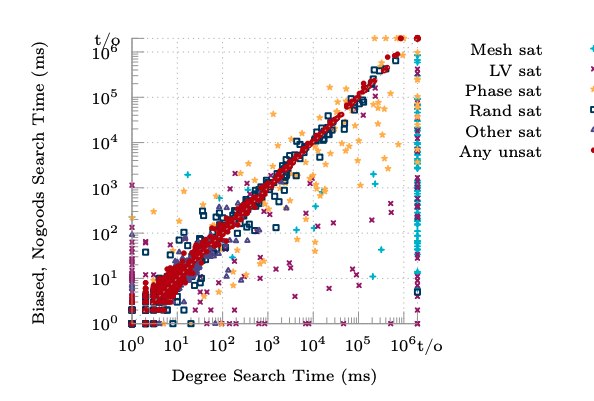
\includegraphics[width=0.7\textwidth]{image-3.png}
    \caption{Degree search time versus biased, nogoods search time, across several instance families (log-log axes; \texttt{t/o} marks the timeout boundary).}
\end{figure}

\end{document}
